%18/09 - Patricia Álvarez
\chapter{Máxima verosimilitud (ML)}
Los métodos probabilísticos se apoyan en la verosimilitud de obtener los datos (un alineamiento múltiple de secuencias) si los linajes hubieran evolucionado de acuerdo con un determinado árbol filogenético (con su topología y longitudes de las ramas) y bajo un determinado modelo de evolución molecular. La máxima verosimilitud intenta responder a la siguiente pregunta: ¿cuál es la probabilidad de observar los datos (el alineamiento), dada una hipótesis (un árbol y un modelo concreto de evolución molecular)? El árbol que hace que los datos sean el resultado más probable es una estimación de máxima verosimilitud de la filogenia. Se hacen dos estimaciones:
\begin{itemize}
\item ¿Cuál de los posibles topologías hace los datos más verosímiles? (NNI, SPR, TBR)
\item Para una topología: ¿qué longitudes de ramas hacen los datos mas verosímiles?
\end{itemize}

La verosimilitud calculada no es la probabilidad de que el árbol sea el correcto, sino lo es de que el árbol estimado generase los datos (si cambian los datos, cambia el árbol). La verosimilitud de un modelo (un árbol filogenético) es igual a la probabilidad de los datos (un alineamiento de secuencias) dada una hipótesis, es decir, un árbol y un modelo de evolución molecular. Esto es una consideración filosófica, ya que la ecuación de verosimilitud no es la probabilidad de que la hipótesis sea correcta en términos absolutos, sino para nuestros datos. La máxima verosimilitud cuenta con una serie de supuestos:
\begin{itemize}
\item Los sitios evolucionan independientemente.
\item Los cambios siguen un modelo de Markov: la probabilidad de que tenga lugar un cambio en un sitio no depende de la historia previa de ese sitio.
\item Los cambios son reversibles en el tiempo.
\end{itemize}

El procedimiento interno calcula la verosimilitud de un alineamiento de dos secuencias, dada una matriz de sustituciones, cierta composición de bases y una longitud concreta para la rama que separa esas secuencias (CED: certain evolutionary distance). Para ello, se calculan todos los eventos posibles. En caso de que haya diferentes longitudes de ramas, para las ramas muy cortas, la probabilidad de que un carácter permanezca inmutable es alta, y la probabilidad de cambio es baja. Para las ramas largas, aumenta la probabilidad de cambio de caracteres y se reduce la probabilidad de mantener estados. Esto genera el problema de \textbf{long branch attraction o atracción de ramas largas}, que ocurre cuando grupos que han evolucionado rápidamente son colocados erróneamente en la base de los árboles filogenéticos al contar con más cambios en sus secuencias.

\begin{figure}[htbp]
\centering
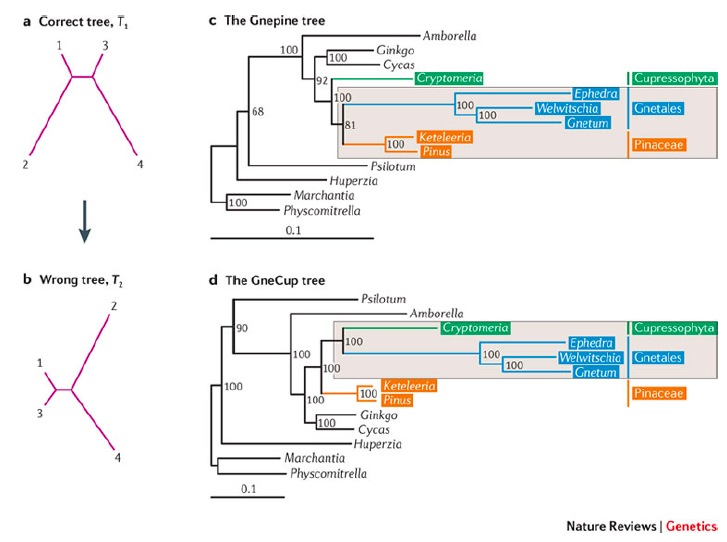
\includegraphics[width=0.5\linewidth]{figs/long-branch-attraction.png}
\caption{La atracción de ramas largas es un fenómeno que se produce cuando se infiere que los linajes que evolucionan rápidamente están estrechamente relacionados, independientemente de sus verdaderas relaciones evolutivas.}
\end{figure}